Find the stationary points of the following functions, stating whether they are local maxima, minima or points of inflexion:
\begin{enumerate}
\item $y=x^2+2$
\item $y = x^3 - 3x+3$
\item $y = x^3 -3x^2 + 3x$ 
\item $y = x^3 + 3x + 3$.
\end{enumerate}
Sketch the graphs of the functions.
\newline
\begin{enumerate}
\item
\[
\frac{dy}{dx} = 2x.
\]
Consequently, this graph has a minimum at $(0,2)$.
\item
\[
\frac{dy}{dx} = 3x^2 - 3.
\]
Consequently this graph has turning points at 
\[
x = \pm 1.
\]
So there is a local maximum at $(-1, 5)$ and a local minimum at $(1,1)$.
\item
\[
\frac{dy}{dx} = 3x^2 -6x +3.
\]
Consequently this graph has turning points at
\[
x = 1\pm\sqrt{36-36} .
\]
Hence this graph has its only turning point at $(1,1)$. The second derivative
\[
y''(1) = 6(1) - 6 = 0
\]
and so this is an inflexion point (which was expected since its the only turning point in a cubic anyway).
\item
\[
\frac{dy}{dx} = 3x^2 + 3.
\]
Since the derivative is strictly positive (from the trivial inequality), there are no turning points in this graph.
\end{enumerate}
\begin{center}
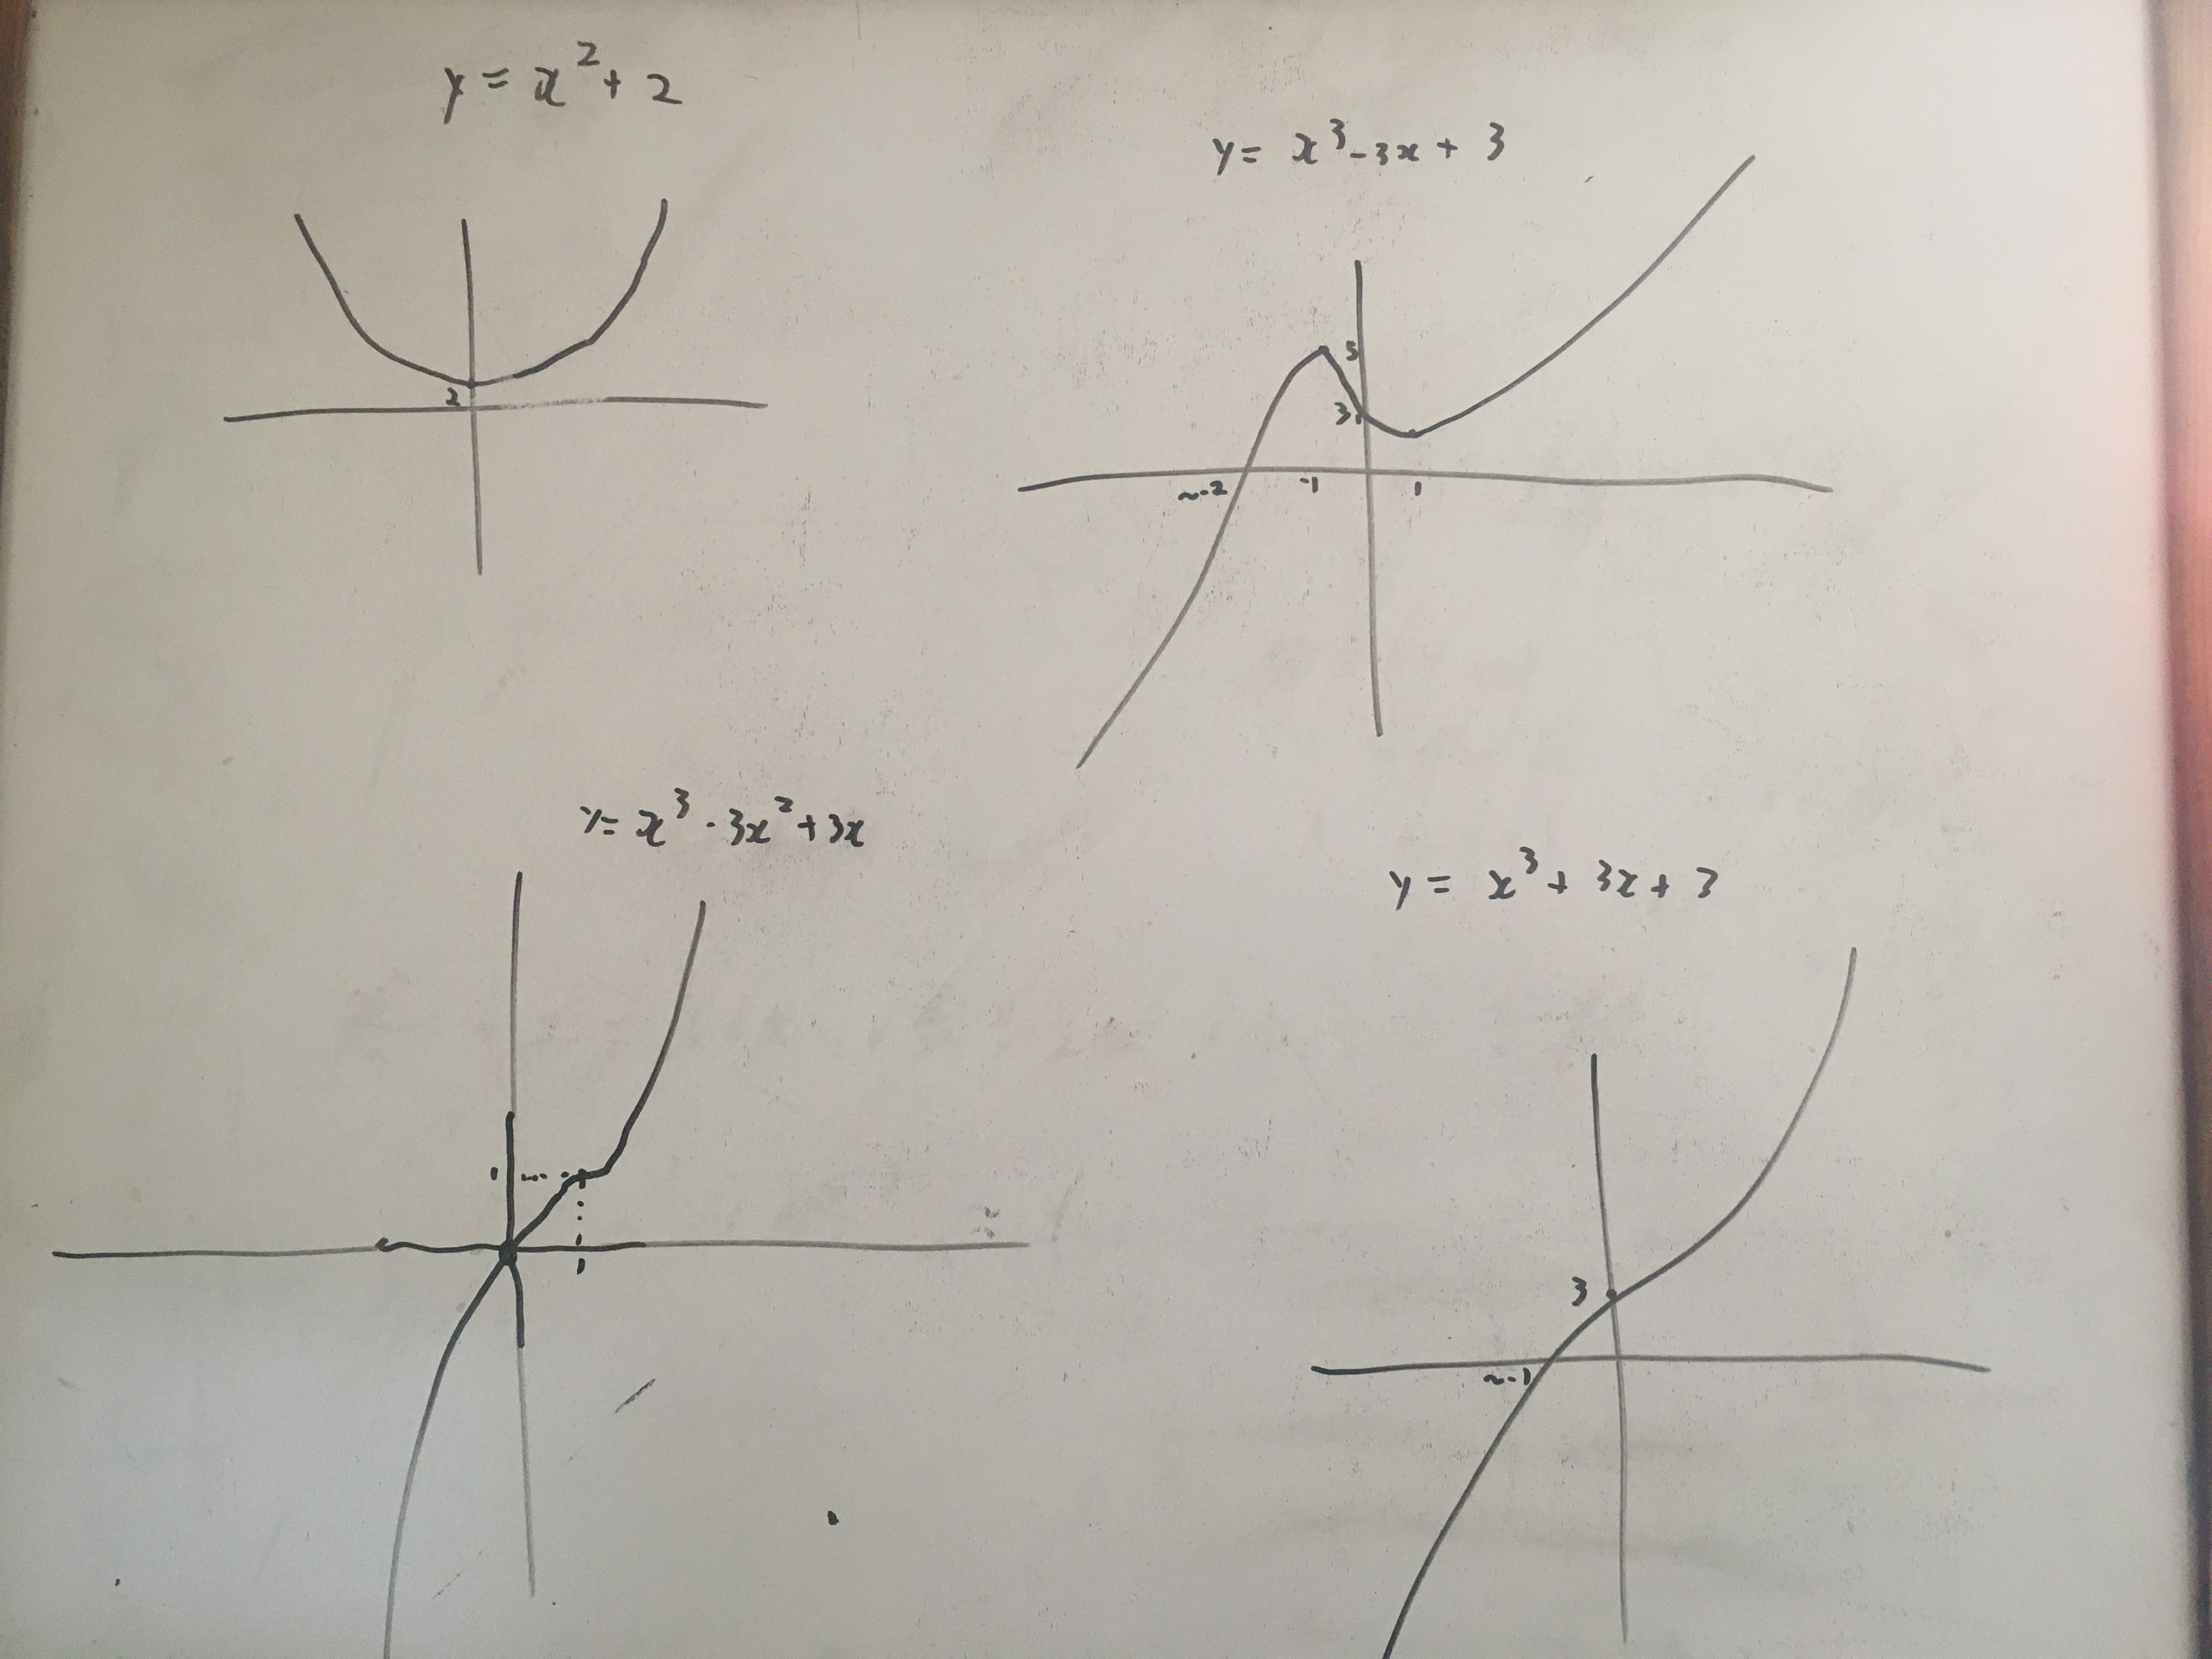
\includegraphics[scale = 0.1]{media/Sketching_from_derivatives}
\end{center}